% !TEX root = SystemTemplate.tex

\chapter{System  and Unit Testing}

This section describes the approach taken with regard to system and unit testing. 

\section{Overview}
The testing approach for this project was a bit different from traditional software testing. We did not have an automated testing framework to run unit tests or regression tests, instead we verified visually when a piece of the project was behaving as expected. This project used many off the shelf hardware and software products where testing the functionality of these pieces has already been done by the manufacturer of that technology. The tests described below allowed us to evaluate whether or not the different subsystems of the UAV were functioning correctly.

\section{Dependencies}
There were no testing frameworks used for this project. All testing was verified manually.

\newpage
\section{Test Setup and Execution}
\subsection{Testing: U-1}
\textbf{As a user, I want to communicate the waypoints to the UAV.}\\
\begin{tabular}{| c | >{\raggedright}m{4cm} | m{4cm} | c |}\hline
	Task No. & Task & Test & Completed\\\hline
	3 & Modify mission communication implementation as necessary & User is able to create mission file with ground control station. & Yes\\\hline
	3 & Modify mission communication implementation as necessary & User is able to load mission file on offboard(ODroid). & Yes\\\hline
	3 & Modify mission communication implementation as necessary & Landing Algorithm on offboard starts after completing last mission. & Yes\\\hline
\end{tabular}

\begin{enumerate}
\item \textbf{TEST: U-1-3-1}\\
\textbf{Relating to Task:} 3\\
\textbf{Task Description:} Modify mission communication implementation as necessary\\
\textbf{Task Test:} User is able to create mission file with ground control station.\\
\textbf{Results:} The team found that QGroundControl worked more reliably, for the purpose of creating navigation files, within a Windows environment. Specifically, the files were created on an install on Windows 10.\par 
The team was able to create a series of missions including takeoff, navigate to waypoints, and landing. The waypoint mission file is exported.

\item \textbf{TEST: U-1-3-2}\\
\textbf{Relating to Task:} 3\\
\textbf{Task Description:} Modify mission communication implementation as necessary\\
\textbf{Task Test:} User is able to load mission file on offboard(ODroid).\\
\textbf{Results:} The team is able to load a mission on the ODroid by connecting directly to the ODroid via network cable. The files are then transferred from a laptop to the ODroid.

\item \textbf{TEST: U-1-3-3}\\
\textbf{Relating to Task:} 3\\
\textbf{Task Description:} Modify mission communication implementation as necessary\\
\textbf{Task Test:} Landing Algorithm on offboard starts after completing last mission.\\
\textbf{Results:} The team has tested that missions will feed the pixhawk via the Mavlink protocol when the pixhawk has indicated that the previous mission parameter has been met. 
\end{enumerate}

\begin{figure}[H]
	\centering
	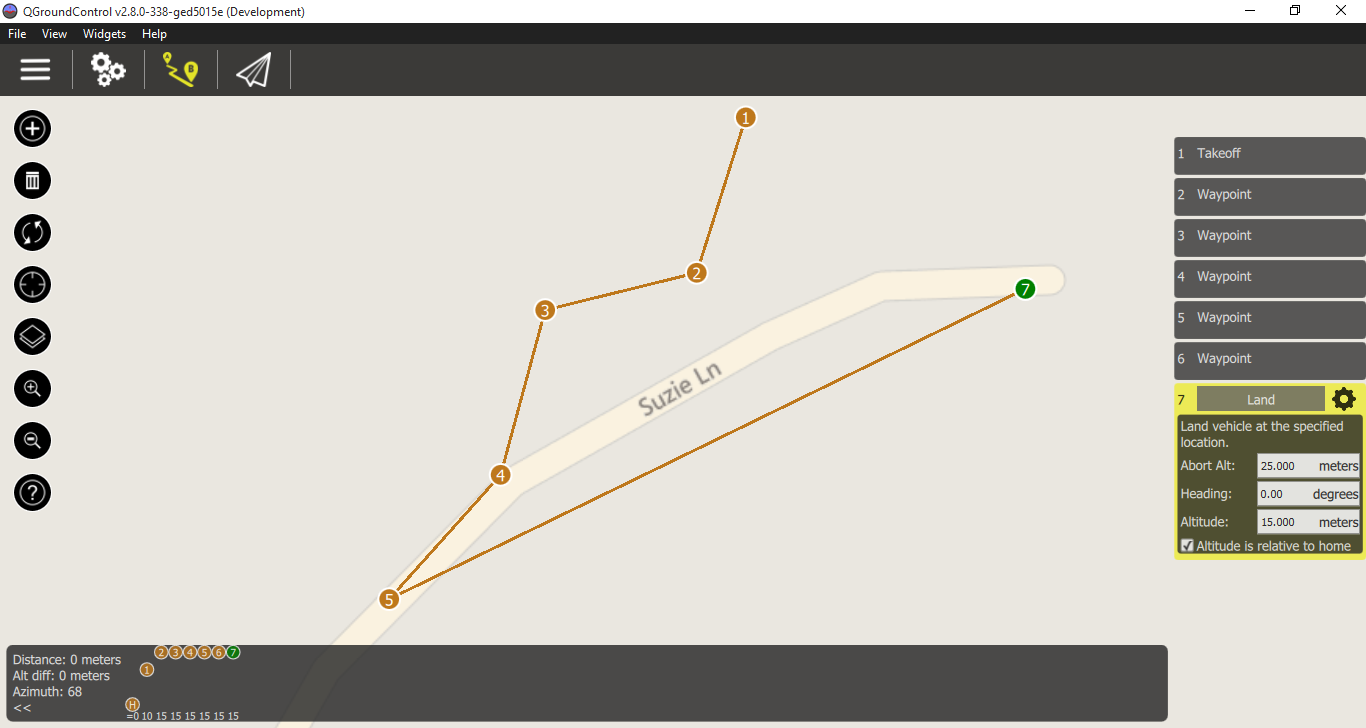
\includegraphics[width=\textwidth]{images/route1.PNG}
	\caption{QGroundControl mission creation.}
\end{figure}

\newpage
\subsection{Testing: O-1}
\textbf{As an owner, I want the UAV to autonomously take-off from the landing pad.}\\
\begin{tabular}{| c | >{\raggedright}m{4cm} | m{4cm} | c |}\hline
	Task No. & Task & Testing & Completed\\\hline
	3 & Modify/Rewrite take-off implementation as necessary
 & FCU recieves take-off mission from mission from offboard control. & Yes\\\hline	
	3 & Modify/Rewrite take-off implementation as necessary
 & FCU executes take-off mission. & Yes\\\hline	
\end{tabular}

\begin{figure}[H]
\centering
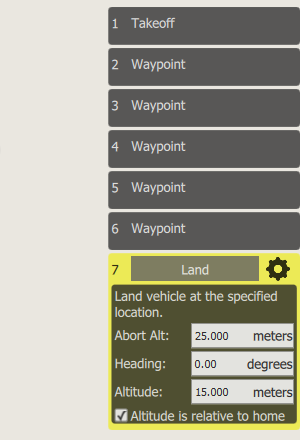
\includegraphics[height=0.5\textwidth]{images/events.PNG}
\caption{QGroundControl showing autonomous takeoff event.}
\label{fig:mission}
\end{figure}

\begin{enumerate}
\item \textbf{TEST: O-1-3-1}\\
\textbf{Relating to Task:} 3\\
\textbf{Task Description:} Modify/Rewrite take-off implementation as necessary \\
\textbf{Task Test:} FCU recieves take-off mission from offboard control..\\
\textbf{Results:} The team successfully tested this by uploading a mission file that included a takeoff event. A sample mission with takeoff event is shown in Figure \ref{fig:mission}.

\item \textbf{TEST: O-1-3-2}\\
\textbf{Relating to Task:} 3\\
\textbf{Task Description:} Modify/Rewrite take-off implementation as necessary\\
\textbf{Task Test:} FCU executes take-off mission\\
\textbf{Results:} The team successfully tested the execution of a takeoff mission by uploading a takeoff mission to the FCU and then allowing the flight controller to run the current mission. 
\end{enumerate}

\newpage
\subsection{Testing: O-2}
\textbf{As an owner, I want the UAV to autonomously navigate through a set of waypoints.}\\
\begin{tabular}{| c | >{\raggedright}m{4cm} | m{4cm} | c |}\hline
	Task No. & Task & Test & Completed\\\hline
	3 & Modify/Rewrite waypoint navigation implementation as necessary & FCU receives navigation missions from offboard control. & Yes\\\hline
	3 & Modify/Rewrite waypoint navigation implementation as necessary & FCU executes navigation in sequence. & Yes\\\hline
	3 & Modify/Rewrite waypoint navigation implementation as necessary & FCU follows, reasonably, the planned navigation. & Yes\\\hline
\end{tabular}

\begin{enumerate}
\item \textbf{TEST: O-2-3-1}\\
\textbf{Relating to Task:} 3\\
\textbf{Task Description:} Modify/Rewrite waypoint navigation implementation as necessary\\
\textbf{Task Test:} FCU receives navigation missions from offboard control.\\
\textbf{Results:} This was successfully tested by simply observing a flight to a single way-point at the end of a driveway.

\item \textbf{TEST: O-2-3-2}\\
\textbf{Relating to Task:} 3\\
\textbf{Task Description:} Modify/Rewrite waypoint navigation implementation as necessary \\
\textbf{Task Test:} FCU executes navigation in sequence.\\
\textbf{Results:} This was verified by creating a multi-way-point mission and ensuring that each way-point was reached in the correct order. For a mission that traced a semicircle in GPS coordinates the UAV traveled along the desired path and made a semicircle before arriving at the final way-point.

\item \textbf{TEST: O-2-3-3}\\
\textbf{Relating to Task:} 3\\
\textbf{Task Description:} Modify/Rewrite waypoint navigation implementation as necessary \\
\textbf{Task Test:} FCU follows, reasonably, the planned navigation.\\
\textbf{Results:} Now that we are sure the way-points are being traversed in order, we must ensure they are being reached accurately. This was verified by having the UAV take off and land on the same exact way-point and marking its takeoff position. The UAV returned and landed with 2 feet of its original takeoff position.
\end{enumerate}

\begin{figure}[H]
\centering
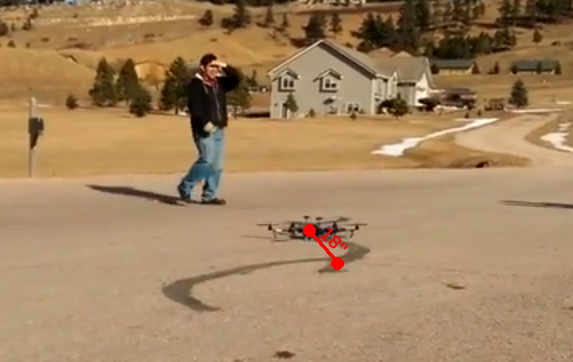
\includegraphics[width=0.7\textwidth]{images/UAVLanding}
\caption{UAV landing error.}
\end{figure}

\newpage
\subsection{Testing: O-3}
\textbf{As an owner, I want the UAV to autonomously return to the location of the landing pad.}\\
\begin{tabular}{| c | >{\raggedright}m{4cm} | m{4cm} | c |}\hline
	Task No. & Task & Test & Completed\\\hline
	3 & Modify navigate to landing waypoint implementation as necessary & FCU receives last navigation mission from offboard control. & Yes\\\hline
	3 & Modify navigate to landing waypoint implementation as necessary & FCU executes navigation mission. & Yes\\\hline
	3 & Modify navigate to landing waypoint implementation as necessary & FCU navigates within a reasonable distance(\textless 10m) to waypoint. & Yes\\\hline
\end{tabular}

\begin{enumerate}
\item \textbf{TEST: O-3-3-1}\\
\textbf{Relating to Task:} 3\\
\textbf{Task Description:} Modify navigate to landing waypoint implementation as necessary\\
\textbf{Task Test:} FCU receives last navigation mission from offboard control.\\
\textbf{Results:} This was successfully tested by simply observing a flight to a single way-point at the end of a driveway.

\item \textbf{TEST: O-3-3-2}\\
\textbf{Relating to Task:} 3\\
\textbf{Task Description:} Modify navigate to landing waypoint implementation as necessary\\
\textbf{Task Test:} FCU executes navigation mission.\\
\textbf{Results:} This was verified by creating a multi-way-point mission and ensuring that each way-point was reached in the correct order. For a mission that traced a semicircle in GPS coordinates the UAV traveled along the desired path and made a semicircle before arriving at the final way-point.

\item \textbf{TEST: O-3-3-3}\\
\textbf{Relating to Task:} 3\\
\textbf{Task Description:} Modify navigate to landing waypoint implementation as necessary\\
\textbf{Task Test:} FCU navigates within a reasonable distance(\textless 10m) to waypoint.\\
\textbf{Results:} In order to test accuracy of a way-point flyby mid mission, we set way-points to landmarks in the environment and had the UAV fly from landmark to landmark. The UAV came well within 10m of each landmark and ends up setting down at the landing zone within 0.5m of the target.
\end{enumerate}

A video showing the successful takeoff, navigation, return and landing is provided \href{https://www.youtube.com/watch?v=wye3LynE1CM}{here}.

\newpage
\subsection{Testing: O-4}
\textbf{As an owner, I want the UAV to autonomously land on the landing pad without damaging the craft}\\
\begin{tabular}{| c | >{\raggedright}m{4cm} | m{4cm} | m{4cm} | m{4cm} |}\hline
	Task No. & Task & Test & Completed\\\hline
	4 & Modify landing pose implementation as necessary & UAV accurately estimates pose of AR tag & Yes\\\hline
	4 & Modify landing pose implementation as necessary & UAV centers over AR tag within (\textless 0.1m). & No\\\hline
	4 & Modify landing pose implementation as necessary & The UAV remains centered during descent within (\textless 0.1m). & No\\\hline
	4 & Modify landing pose implementation as necessary & The UAV lands without damaging craft or legs. & No\\\hline
\end{tabular}

\begin{enumerate}
\item \textbf{TEST: O-4-4-1}\\
\textbf{Relating to Task:} 4\\
\textbf{Task Description:} Modify landing pose implementation as necessary\\
\textbf{Task Test:} UAV accurately estimates pose of AR tag.\\
\textbf{Results:} Using AR Track ALVAR, an AR Tag can be seen from about 15 feet away and its pose estimated very accurately.

\begin{figure}[H]
\centering
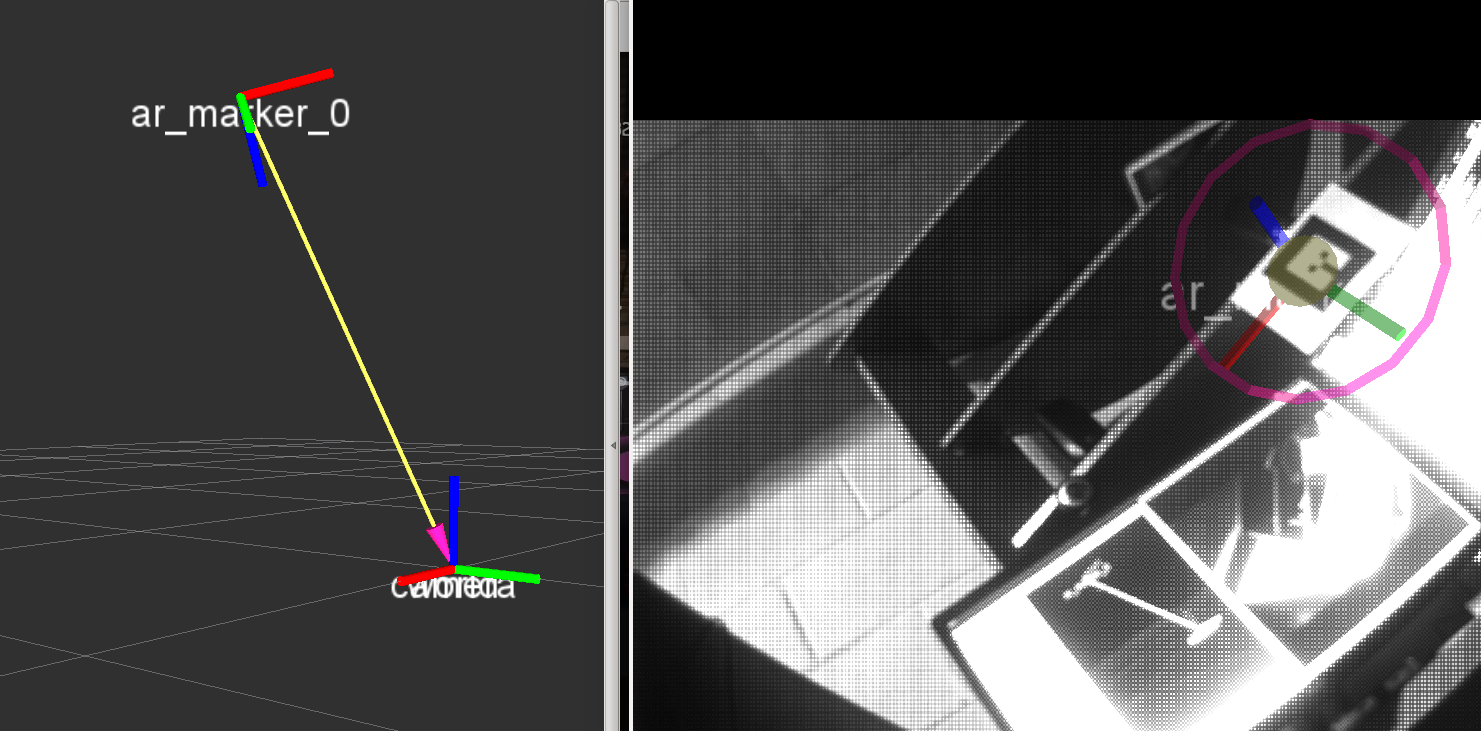
\includegraphics[width=\textwidth]{images/poseEstimation.png}
\caption{AR Tag tracking with AR Track ALVAR}
\label{fig:artrack}
\end{figure}

\item \textbf{TEST: O-4-4-2}\\
\textbf{Relating to Task:} 4\\
\textbf{Task Description:} Modify landing pose implementation as necessary\\
\textbf{Task Test:} UAV centers over AR tag within (\textless 0.1m).\\
\textbf{Results:} Not tested.

\item \textbf{TEST: O-4-4-3}\\
\textbf{Relating to Task:} 4\\
\textbf{Task Description:} Modify landing pose implementation as necessary\\
\textbf{Task Test:} The UAV remains centered during descent within (\textless 0.1m).\\
\textbf{Results:} Not tested.

\item \textbf{TEST: O-4-4-4}\\
\textbf{Relating to Task:} 4\\
\textbf{Task Description:} Modify landing pose implementation as necessary\\
\textbf{Task Test:} The UAV lands without damaging craft or legs.\\
\textbf{Results:} The UAV was able to land without damaging the craft under control of the FCU. Offboard control of the landing was not tested.
\end{enumerate}

\newpage
\subsection{Testing: O-5}
\textbf{As an owner, I want the UAV to autonomously land on the landing pad with the correct orientation.}\\
\begin{tabular}{| c | >{\raggedright}m{4cm} | m{4cm} | m{4cm} |}\hline
	Task No. & Task & Test & Completed\\\hline
		4 & Modify landing orientation implementation as necessary & UAV accurately estimates the orientation of AR tag & Yes\\ \hline
		4 & Modify landing orientation implementation as necessary & UAV changes orientation to align with AR tag, within 15$\deg$ & No\\ \hline
		4 & Modify landing orientation implementation as necessary & UAV maintains correct orientation during descent within 15$\deg$ & No\\ \hline
\end{tabular}

\begin{enumerate}
\item \textbf{TEST: O-5-4-1}\\
\textbf{Relating to Task:} 3\\
\textbf{Task Description:} Modify landing orientation implementation as necessary\\
\textbf{Task Test:} UAV accurately estimates the orientation of AR tag.\\
\textbf{Results:} See Figure \ref{fig:artrack} for results of AR Tag tracking.

\item \textbf{TEST: O-5-4-2}\\
\textbf{Relating to Task:} 3\\
\textbf{Task Description:} Modify landing orientation implementation as necessary\\
\textbf{Task Test:} UAV changes orientation to align with AR tag, within 15$\deg$.\\
\textbf{Results:} Not tested.

\item \textbf{TEST: O-5-4-3}\\
\textbf{Relating to Task:} 3\\
\textbf{Task Description:} Modify landing orientation implementation as necessary\\
\textbf{Task Test:} UAV maintains correct orientation during descent within 15$\deg$.\\
\textbf{Results:}  Not tested.
\end{enumerate}
